\documentclass[letterpaper, 10pt]{article}
\usepackage{amsmath}
\usepackage{tikz}
\usepackage{amsmath}
\usetikzlibrary{bayesnet}
\usetikzlibrary{shapes.gates.logic.US,trees,positioning,arrows}
\usetikzlibrary{shapes,snakes}
\usetikzlibrary{trees}
\usepackage{amssymb}

\begin{document}

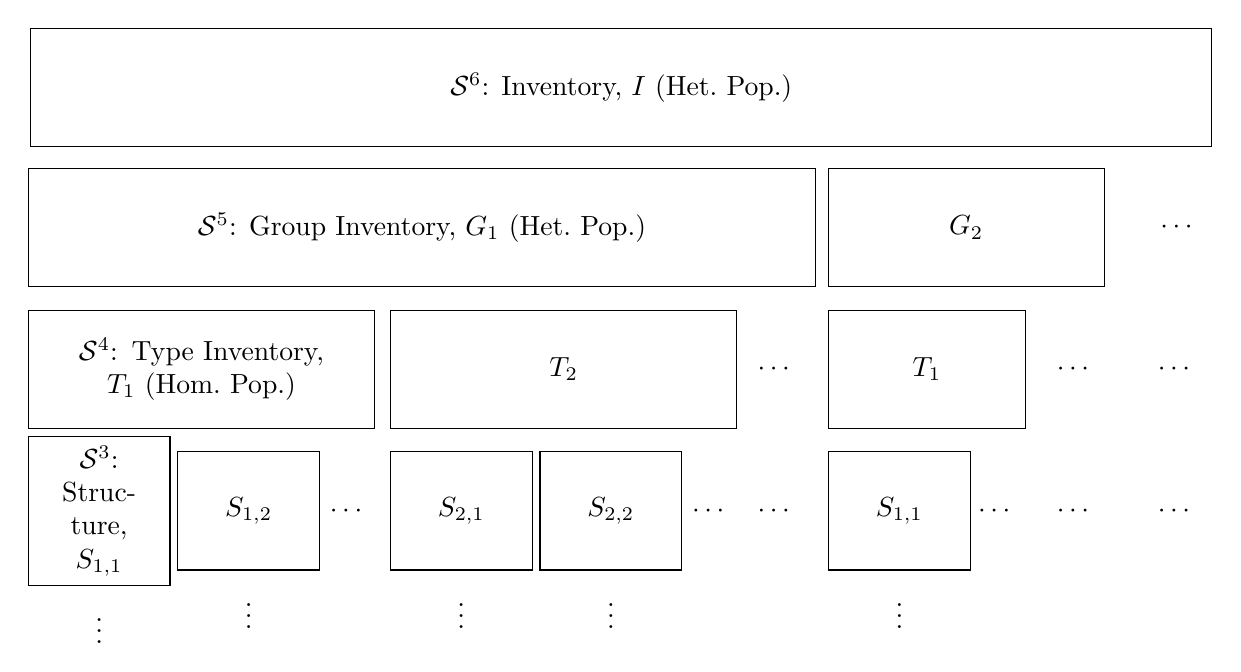
\begin{tikzpicture}
	
	\node[rectangle,draw=black,minimum width=15cm,minimum height=1.5cm] (S6) {$\mathcal{S}^{6}$: Inventory, $I$ (Het.\ Pop.)} ;
	\node[const, below=1cm of S6] (temp1) { } ; % Reference node
	\node[rectangle, left=-2.5cm of temp1, draw=black,minimum width=10cm,minimum height=1.5cm] (S51) {$\mathcal{S}^{5}$: Group Inventory, $G_1$ (Het.\ Pop.)} ;
	\node[rectangle, right=2.6cm of temp1, draw=black,minimum width=3.5cm,minimum height=1.5cm] (S52) {$G_2$} ;
	\node[const, right=0.7cm of S52] (Gcont) {$\cdots$} ;
	\node[const, below=1.75cm of temp1] (temp2) { } ; % Reference node
	\node[rectangle, left=-1.5cm of temp2, draw=black,minimum width=4.4cm,minimum height=1.5cm] (S42) {$T_2$} ;
	\node[rectangle, left=3.1cm of temp2, draw=black,minimum width=4.4cm,minimum height=1.5cm,text width=4cm,align=center] (S41) {$\mathcal{S}^{4}$: Type Inventory, $T_1$ (Hom.\ Pop.)} ;
	\node[const, right=1.7cm of temp2] (Tcont1) {$\cdots$} ;
	\node[rectangle, right=2.6cm of temp2, draw=black,minimum width=2.5cm,minimum height=1.5cm] (S43) {$T_1$} ;
	\node[const, right=5.5cm of temp2] (Tcont2) {$\cdots$} ;
	\node[const, right=0.8cm of Tcont2] (Tcont3) {$\cdots$} ;
	\node[const, below=1.75 of temp2] (temp3) { } ; % Reference node
	\node[rectangle, left=3.8cm of temp3,draw=black,minimum width=1.8cm,minimum height=1.5cm] (S32) { $S_{1,2}$} ;
	\node[rectangle, left=5.7cm of temp3,draw=black,minimum width=1.8cm,minimum height=1.5cm,text width=1.5cm,align=center] (S31) {$\mathcal{S}^{3}$: Structure, $S_{1,1}$} ;
	\node[const, left=3.2cm of temp3] (Scont1) {$\cdots$} ;
	\node[rectangle, left=-0.8cm of temp3,draw=black,minimum width=1.8cm,minimum height=1.5cm] (S34) { $S_{2,2}$} ;
	\node[rectangle, left=1.1cm of temp3,draw=black,minimum width=1.8cm,minimum height=1.5cm] (S33) { $S_{2,1}$} ;
	\node[const, left=-1.4cm of temp3] (Scont2) {$\cdots$} ;
	\node[const, right=1.7cm of temp3] (Scont3) {$\cdots$} ;
	\node[rectangle, right=2.6cm of temp3,draw=black,minimum width=1.8cm,minimum height=1.5cm] (S35) { $S_{1,1}$} ;
	\node[const, right=4.5cm of temp3] (Scont4) {$\cdots$} ;
	\node[const, right=5.5cm of temp3] (Scont5) {$\cdots$} ;
	\node[const, right=0.8cm of Scont5] (Scont6) {$\cdots$} ;
	\node[const, below=0.2cm of S31] (Ccont1) {$\vdots$} ;
	\node[const, below=0.2cm of S32] (Ccont2) {$\vdots$} ;
	\node[const, below=0.2cm of S33] (Ccont3) {$\vdots$} ;
	\node[const, below=0.2cm of S34] (Ccont4) {$\vdots$} ;
	\node[const, below=0.2cm of S35] (Ccont5) {$\vdots$} ;
	
\end{tikzpicture}

\end{document}